\documentclass[12pt]{article}

\usepackage[margin=50pt]{geometry}
\usepackage{amsmath}
\usepackage{graphicx}
\usepackage{xcolor}

\usepackage{titling}
\newcommand{\subtitle}[1]{%
  \posttitle{%
    \par\end{center}
    \begin{center}\large#1\end{center}
    \vskip0.5em}%
}

\graphicspath{/images}
\geometry{footskip=0.8cm}

\title{Linear Programming}
\subtitle{Graded Assignments 1}
\author{Thomas Vroom (6291496)}

\begin{document}
\maketitle

%
% Exercise 1
%
\section{Modelling}
The decision variables for this problem are the amount of red, green and blue sand (in kg) per bucket:

\begin{table}[h]
  \centering
  \begin{tabular}{l|lllll}
   & $b_1$ & $b_2$ & $b_3$ & $b_4$ & $b_5$ \\ \hline
  kg of red sand & $x_{1,r}$ & $x_{2,r}$ & $x_{3,r}$ & $x_{4,r}$ & $x_{5,r}$ \\
  kg of blue sand & $x_{1,b}$ & $x_{2,b}$ & $x_{3,b}$ & $x_{4,b}$ & $x_{5,b}$ \\
  kg of green sand & $x_{1,g}$ & $x_{2,g}$ & $x_{3,g}$ & $x_{4,g}$ & $x_{5,g}$
  \end{tabular}
\end{table}

\noindent
For example, $x_{2,b}$ represents the amount of blue sand in bucket 2 (in kg), etc.

\subsection*{Objective Function}
The goal of the LP is to \textbf{minimize} the following function:
\[ Z = (x_{1,r} + x_{2,r} + x_{3,r} + x_{4,r} + x_{5,r}) \cdot 2.5 + (x_{1,b} + x_{2,b} + x_{3,b} + x_{4,b} + x_{5,b}) \cdot 2 + (x_{1,g} + x_{2,g} + x_{3,g} + x_{4,g} + x_{5,g}) \]

\subsection*{Constraints}
Our supplier only has a limited amount of sand available:
\[ x_{1,r} + x_{2,r} + x_{3,r} + x_{4,r} + x_{5,r} \leq 30 \]
\[ x_{1,b} + x_{2,b} + x_{3,b} + x_{4,b} + x_{5,b} \leq 20 \]
\[ x_{1,g} + x_{2,g} + x_{3,g} + x_{4,g} + x_{5,g} \leq 25 \]

\noindent
No bucket should be overloaded beyond its maximum capacity:
\[ x_{1,r} + x_{1,b} + x_{1,g} \leq 7 \]
\[ x_{2,r} + x_{2,b} + x_{2,g} \leq 8 \]
\[ x_{3,r} + x_{3,b} + x_{3,g} \leq 5 \]
\[ x_{4,r} + x_{4,b} + x_{4,g} \leq 20 \]
\[ x_{5,r} + x_{5,b} + x_{5,g} \leq 15 \]

\newpage
\noindent
Each bucket should be at least half-filled:
\[ x_{1,r} + x_{1,b} + x_{1,g} \geq 3.5 \]
\[ x_{2,r} + x_{2,b} + x_{2,g} \geq 4 \]
\[ x_{3,r} + x_{3,b} + x_{3,g} \geq 2.5 \]
\[ x_{4,r} + x_{4,b} + x_{4,g} \geq 10 \]
\[ x_{5,r} + x_{5,b} + x_{5,g} \geq 7.5 \]

\noindent
In each bucket, the amount of red sand used should be at least half of the total amount of sand in the bucket:
\[ x_{1,r} \geq x_{1,b} + x_{1,g} \]
\[ x_{2,r} \geq x_{2,b} + x_{2,g} \]
\[ x_{3,r} \geq x_{3,b} + x_{3,g} \]
\[ x_{4,r} \geq x_{4,b} + x_{4,g} \]
\[ x_{5,r} \geq x_{5,b} + x_{5,g} \]

\noindent
For each two adjacent buckets, the total amount of blue sand in the two buckets should be at least 5kg:
\[ x_{1,b} + x_{2,b} \geq 5 \]
\[ x_{2,b} + x_{3,b} \geq 5 \]
\[ x_{3,b} + x_{4,b} \geq 5 \]
\[ x_{4,b} + x_{5,b} \geq 5 \]

\noindent
Lastly, a bucket cannot have a negative amount of sand in it (nonnegativity constraints):
\[ x_{i,j} \geq 0, \text{ for all } i = \{1, 2, 3, 4, 5\}, j = \{\text{r}, \text{b}, \text{g}\} \]

%
% Exercise 2
%
\newpage
\section{Simplex Method}
Consider the following linear program:
\begin{align*}
  &\mathrm{max} \quad Z = 3x_1 + x_2 + 2x_3 \\[2pt]
  &\mathrm{s.t.} \quad 
  \begin{array}[t]{r c r c r c r c r c r c r c}
      -x_1 & + & 2x_2 & - & x_3 & + & \textcolor{red}{x_4} & & & & & = & 20 \\
      2x_1 & - & 4x_2 & + & 2x_3 & & & + & \textcolor{red}{x_5} & & & = & 30 \\
      3x_1 & + & 3x_2 & + & x_3 & & & & & + & \textcolor{red}{x_6} & = & 25
  \end{array}\\
  &\mathrm{and} \quad x_j \geq 0
\end{align*}

\noindent
Where the \textcolor{red}{red}-colored variables $\textcolor{red}{x_4}, \textcolor{red}{x_5}, \textcolor{red}{x_6}$ are slack variables.

\subsection{Solve this LP using the Simplex method}
We can transform the above LP into the following tableau:

\begin{equation*}
  \begin{array}{cc|r|rrrrrr|c}
            &     & Z & x_1 & x_2 & x_3 & x_4 & x_5 & x_6 & \text{RHS} \\ \hline
        z   & (0) & 1 &  -3 &  -1 &  -2 &   0 &   0 &   0 & 0 \\
        x_4 & (1) & 0 &  -1 &   2 &  -1 &   1 &   0 &   0 & 20 \\
        x_5 & (2) & 0 &   2 &  -4 &   2 &   0 &   1 &   0 & 30 \\
        x_6 & (3) & 0 &   3 &   3 &   1 &   0 &   0 &   1 & 25
  \end{array}
\end{equation*}

\noindent
Here $x_1$ is the entering variable, as -3 is the most negative value in the top row.
We can find the leaving variable by applying the minimum ratio test:

\begin{itemize}
  \item row $(2)$: $\frac{30}{2} = 15$
  \item row $(3)$: $\frac{25}{3} = 8\frac{1}{3}$
\end{itemize}

\noindent
$8\frac{1}{3} < 15$, thus $x_6$ (row $(3)$) is the leaving variable.

\noindent
\\
By applying Gaussian elimination, we reach the following tableau:

\begin{equation*}
  \begin{array}{cc|r|rrrrrr|c}
            &     & Z & x_1 & x_2 &           x_3 & x_4 & x_5 &           x_6 & \text{RHS} \\ \hline
        z   & (0) & 1 &   0 &   2 &            -1 &   0 &   0 &             1 & 25 \\
        x_4 & (1) & 0 &   0 &   3 &  -\frac{2}{3} &   1 &   0 &   \frac{1}{3} & 28\frac{1}{3} \\
        x_5 & (2) & 0 &   0 &  -6 &  1\frac{1}{3} &   0 &   1 &  -\frac{2}{3} & 13\frac{1}{3} \\
        x_1 & (3) & 0 &   1 &   1 &   \frac{1}{3} &   0 &   0 &   \frac{1}{3} & 8\frac{1}{3}
  \end{array}
\end{equation*}

\noindent
Here $x_3$ is the entering variable, as -1 is the most negative value in the top row.
We can find the leaving variable by applying the minimum ratio test:

\begin{itemize}
  \item row $(2)$: $\frac{13\frac{1}{3}}{1\frac{1}{3}} = 10$
  \item row $(3)$: $\frac{8\frac{1}{3}}{\frac{1}{3}} = 25$
\end{itemize}

\noindent
$10 < 25$, thus $x_5$ (row $(2)$) is the leaving variable.

\noindent
\\
By applying Gaussian elimination, we reach the following tableau:

\newpage
\begin{equation*}
  \begin{array}{cc|r|rrrrrr|c}
            &     & Z & x_1 &           x_2 & x_3 & x_4 &          x_5 &          x_6 & \text{RHS} \\ \hline
        z   & (0) & 1 &   0 & -2\frac{1}{2} &   0 &   0 &  \frac{3}{4} &  \frac{1}{2} & 35 \\
        x_4 & (1) & 0 &   0 &             0 &   0 &   1 &  \frac{1}{2} &            0 & 35 \\
        x_3 & (2) & 0 &   0 & -4\frac{1}{2} &   1 &   0 &  \frac{3}{4} & -\frac{1}{2} & 10 \\
        x_1 & (3) & 0 &   1 &  2\frac{1}{2} &   0 &   0 & -\frac{1}{4} &  \frac{1}{2} & 5
  \end{array}
\end{equation*}

\noindent
Here $x_2$ is the entering variable, as $-2\frac{1}{2}$ is the most negative value in the top row.
$x_1$ is the leaving variable, as $2\frac{1}{2}$ is the only postive non-zero element in the column of $x_2$.

\noindent
\\
By applying Gaussian elimination, we reach the following tableau:

\begin{equation*}
  \begin{array}{cc|r|rrrrrr|c}
            &     & Z &          x_1 & x_2 & x_3 & x_4 &          x_5 &          x_6 & \text{RHS} \\ \hline
        z   & (0) & 1 & 1\frac{2}{3} &   0 &   0 &   0 &  \frac{1}{3} & 1\frac{1}{3} & 40 \\
        x_4 & (1) & 0 &            0 &   0 &   0 &   1 &  \frac{1}{2} &            0 & 35 \\
        x_3 & (2) & 0 &            3 &   0 &   1 &   0 &            0 &            1 & 19 \\
        x_2 & (3) & 0 &  \frac{2}{3} &   1 &   0 &   0 & -\frac{1}{6} &  \frac{1}{3} & 2
  \end{array}
\end{equation*}

\noindent
Now we have reached optimality, as there are no negative values in the top row.
The value of the objective function is:

\[ Z = 40 \]

\noindent
And the variable assignment is:

\[ (x_1, x_2, x_3, x_4, x_5, x_6) = (0, 2, 19, 35, 0, 0) \]

\subsection{Which variables are (non)basic?}
$\{ x_2, x_3, x_4 \}$ is the basis, so $x_2$, $x_3$ and $x_4$ are basic variables.
The other variables, $\{ x_1, x_5, x_6 \}$, are nonbasic variables. 

%
% Exercise 3
%
\newpage
\section{Degeneracy}
We are given a linear program with two non-negative decision variables, $x_1$ and $x_2$, and two functional constraints:

\[ x_1 \leq 1 \]
\[ x_1 + x_2 \leq 2 \]

\subsection{List all the basic feasible solutions of this program}
We can visualize this program as follows: 

\begin{figure}[h]
  \centering
  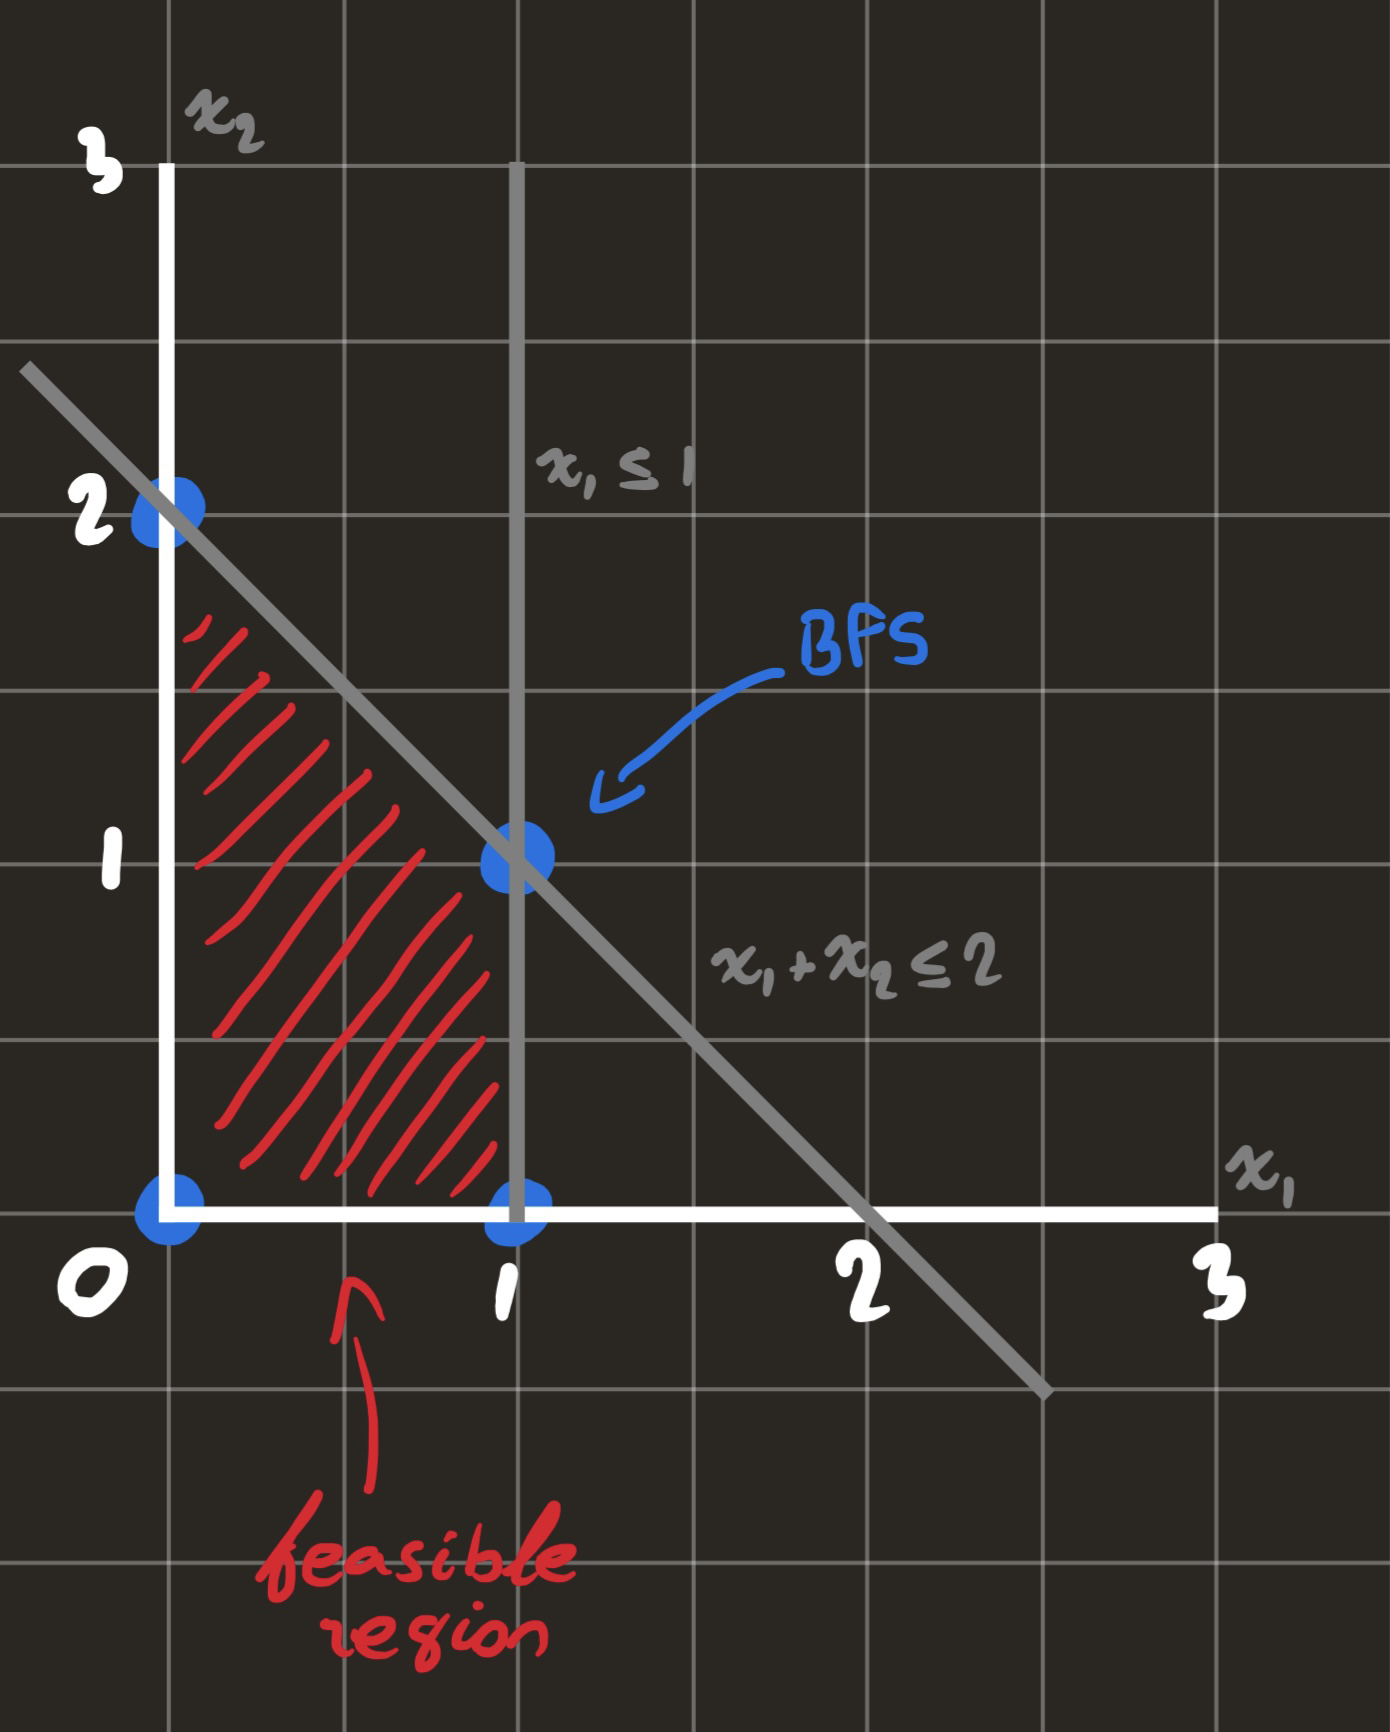
\includegraphics[scale=0.125]{images/sketch.jpg}
\end{figure}

\noindent
The basic feasible solutions are represented by the (\textcolor{blue}{blue}-colored) corner points of the feasible region.
If we rewrite the constraints to include slack variables:

\[ x_1 + \textcolor{red}{x_3} = 1 \]
\[ x_1 + x_2 + \textcolor{red}{x_4} = 2 \]

\noindent
We can read off all the basic feasible solutions, with their respective basis' and tight constraints as follows:

\begin{itemize}
  \item $(x_1, x_2, x_3, x_4) = (0, 0, 1, 2)$, with basis $\{ x_3, x_4 \}$. The tight constraints here are the non-negativity constraints of $x_1$ and $x_2$.
  \item $(x_1, x_2, x_3, x_4) = (0, 2, 1, 0)$, with basis $\{ x_2, x_3 \}$. The tight constraints here are the non-negativity constraint of $x_1$ and $x_1 + x_2 \leq 2$.
  \item $(x_1, x_2, x_3, x_4) = (1, 0, 0, 1)$, with basis $\{ x_1, x_4 \}$. The tight constraints here are the non-negativity constraint of $x_2$ and $x_1 \leq 1$.
  \item $(x_1, x_2, x_3, x_4) = (1, 1, 0, 0)$, with basis $\{ x_1, x_2 \}$. The tight constraints here are $x_1 \leq 1$ and $x_1 + x_2 \leq 2$.
\end{itemize}

\newpage
\subsection{How many basic solutions does this program have?}
The basic solutions of this program are represented by \textit{all} corner points of the visualization above.
This includes the basic feasible solutions shown above, as well as the corner point $(x_1, x_2, x_3, x_4) = (2, 0, -1, 0)$.
This makes for a total of 5 basic solutions.

\subsection{Add a third constraint such that the resulting linear program has at least one degenerate BFS}
One way to do this is to introduce a new constraint boundary that intercepts the other constraint boundaries at the same BFS.
This BFS will then become degenerate.
The constraint we will introduce is:

\[ x_2 \leq 1 \]

\noindent
Which can also be written as:

\[ x_2 + \textcolor{red}{x_5} = 1 \]

\noindent
We can visualize this program as follows: 

\begin{figure}[h]
  \centering
  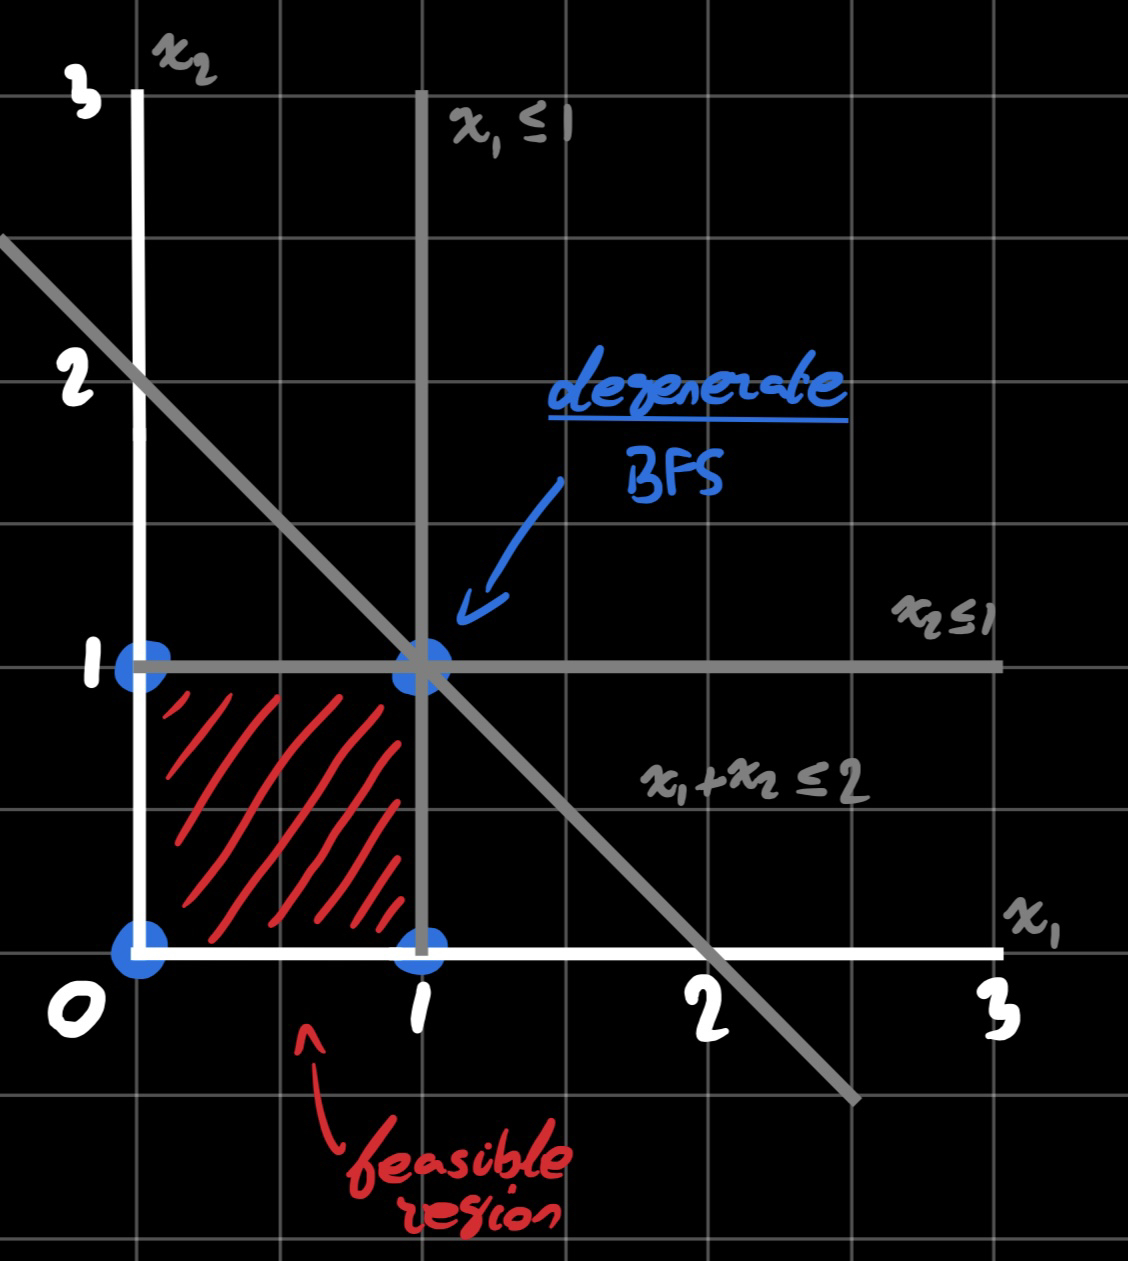
\includegraphics[scale=0.2]{images/sketch2.png}
\end{figure}

\noindent
The BFS at the intersection of the constraint boundaries represents the solution $(x_1, x_2, x_3, x_4, x_5) = (1, 1, 0, 0, 0)$.
This BFS is degenerate, because it has a basic variable that is equal to 0.

\end{document}
